\subsubsection{Listar}

  \paragraph{}Para mostrar esta lista, es necesario establecer el centro para
  el que mostrar las calificaciones por convocatoria disponibles. Para ello,
  habrá que elegir el centro en la lista desplegable que se muestra en la figura
  \ref{capturaPantallaSelectCentro}.

  \paragraph{}También será necesario elegir la titulación a la que pertenecen
  las calificaciones, por lo que se elegirá entre las opciones de una lista
  desplegable, siguiendo el mismo mecanismo que para seleccionar centro. Se
  puede ver una captura de la selección de titulación en la figura
  \ref{capturaPantallaSelectTitulacion}.

  \paragraph{}Además, habrá que seleccionar la asignatura para la cual se
  listarán las calificaciones disponibles. Al igual que para la selección de
  centro y de titulación, se seleccionará a través de una lista desplegable con
  las asignaturas disponibles. La figura \ref{capturaPantallaSelectAsignatura}
  muestra una captura de pantalla de esta ventana.

  \paragraph{}Es necesario también elegir el curso académico existente para el
  que se realizará el listado de calificaciones. Se puede ver una captura de
  pantalla de esta ventana en la figura
  \ref{capturaPantallaSelectCursoAcademicoAsignatura}.

  \paragraph{}Por último, habrá que elegir la matrícula para la que establecer
  la calificación, seleccionándola por el mismo procedimiento antes comentado.
  Se puede ver una captura de pantalla de la ventana de selección de matrícula
  en la figura \ref{capturaPantallaSelectMatricula}.

  \begin{figure}[!ht]
    \begin{center}
      \fbox{
      
\includegraphics[scale=0.55]{4.Funcionamiento_Aplicacion/4.3.Gestion/4.3.1.Administrador_Principal/4.3.1.14.CalificacionConvocatoria/select_matricula.png}
      }
      \caption{Captura de pantalla de la lista desplegable para seleccionar matrícula para el usuario \textit{Administrador principal}.}
      \label{capturaPantallaSelectMatricula}
    \end{center}
  \end{figure}

  \paragraph{}Nótese que si no existieran elementos disponibles en el sistema,
  la lista desplegable aparecería vacía. Por tanto, se proporciona al usuario
  un icono, representado por una cruz verde, para añadir nuevos elementos al
  sistema. Este icono es el mostrado en la figura \ref{capturaBotonAdd}. Al
  pulsar dicho botón, aparecerá la ventana de creación de un nuevo elemento.

  \paragraph{}Una vez seleccionados el centro, la titulación, la asignatura,
  el curso académico y la matrícula, se muestra la lista completa de
  calificaciones que aparecen en el sistema. La figura
  \ref{capturaPantallaListaCalificacionesAdminPrincipal} muestra una captura de
  pantalla de la lista de calificaciones por convocatoria.

  \begin{figure}[!ht]
    \begin{center}
      \fbox{
      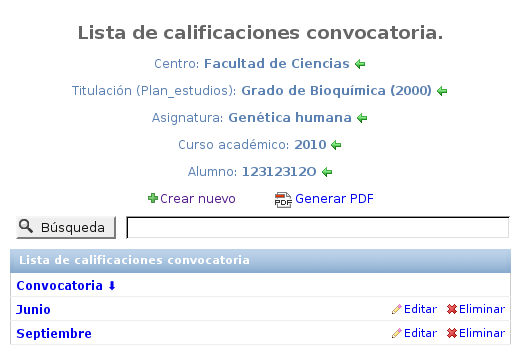
\includegraphics[scale=0.55]{4.Funcionamiento_Aplicacion/4.3.Gestion/4.3.1.Administrador_Principal/4.3.1.14.CalificacionConvocatoria/lista_calificaciones.png}
      }
      \caption{Captura de pantalla de la lista de calificaciones por convocatoria para el usuario \textit{Administrador principal}.}
      \label{capturaPantallaListaCalificacionesAdminPrincipal}
    \end{center}
  \end{figure}

  \paragraph{}Si se quisiera refinar el listado de elementos mostrados, es
  posible seleccionar nuevos parámetros pulsando el icono \textit{Seleccionar}
  que aparece al lado de cada elemento. Este icono aparece en la figura
  \ref{capturaBotonSeleccionar}.
